\ifdefined\gkver\else\def\gkver{student}\fi
\documentclass[\gkver]{gaokaozhenti}
\newcommand{\ccnum}[1]{{\fontspec{Noto Sans CJK JP}#1}}
\begin{document}

\chapter{2015年天津理综}
%% paperType: 理综物理部分

\begin{enumerate}
\item
%% number: 1
%% paperName: 2015年天津理综第 1 题 6 分
%% typeId: 1
%% type: 单选题
%% chapter: 其他
%% point: 物理学史
%% method: 无
%% score: 6
%% degree: 650
%% duplicateId: 0
%% body:
物理学重视逻辑，崇尚理性，其理论总是建立在对事实观察的基础上，下列说法正确的是\xzanswer{A}
\fourchoices[answer=A]
{天然放射现象说明原子核内部是有结构的}
{电子的发现使人认识到原子具有核式结构}
{$\alpha$粒子散射实验的重要发现是电荷是量子化的}
{密立根油滴实验表明核外电子的轨道是不连续的}
%% answer: A
%% memo:
\memoanswer{
	本题原卷及材料中未提供详解，待补充。
}

\item
%% number: 2
%% paperName: 2015年天津理综第 2 题 6 分
%% typeId: 1
%% type: 单选题
%% chapter: 光学
%% point: 光的折射
%% method: 无
%% score: 6
%% degree: 650
%% duplicateId: 0
%% body:
中国古人对许多自然现象有深刻认识，唐人张志和在《玄真子·涛之灵》中写道：“雨色映日而为虹”。从物理学的角度看，虹是太阳光经过雨滴的两次折射和一次反射形成的，右图是彩虹成因的简化示意图，其中 a、b 是两种不同频率的单色光，则两光\xzanswer{C}

\onepicture[h=3.2cm]{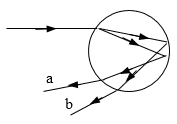
\includegraphics{figs/02.png}}

\fourchoices[answer=C]
{在同种玻璃中传播，a 光的传播速度一定大于 b 光}
{以相同角度斜射到同一玻璃板透过平行表面后，b 光侧移量大}
{分别照射同一光电管，若 b 光能引起光电效应，a 光一定也能}
{以相同的入射角从水中射入空气，在空气中只能看到一种光时，一定是 a 光}
%% answer: C
%% memo:
\memoanswer{
	本题原卷及材料中未提供详解，待补充。
}

\item
%% number: 3
%% paperName: 2015年天津理综第 3 题 6 分
%% typeId: 1
%% type: 单选题
%% chapter: 机械波
%% point: 波与振动图象
%% method: 无
%% score: 6
%% degree: 450
%% duplicateId: 0
%% body:
图甲为一列简谐横波在某一时刻的波形图，a、b 两质点的横坐标分别为 $x_{a}=2\Um$ 和 $x_{b}=6\Um$，图乙为质点 b 从该时刻开始计时的振动图象，下列说法正确的是\xzanswer{D}

\twopicture[numA={甲}, numB={乙}, labelA=2015天津理综03a, labelB=2015天津理综03b, hA=3.6cm, hB=3.6cm]
{figs/03a.png}
{figs/03b.png}

\fourchoices[answer=D]
{该波沿 $+x$ 方向传播，波速为 $1\Ums$}
{质点 a 经过 $4\Us$ 振动的路程为 $4\Um$}
{此时刻质点 a 的速度沿 $+y$ 方向}
{质点 a 在 $t=2\Us$ 时速度为零}
%% answer: D
%% memo:
\memoanswer{
	本题原卷及材料中未提供详解，待补充。
}

\item
%% number: 4
%% paperName: 2015年天津理综第 4 题 6 分
%% typeId: 1
%% type: 单选题
%% chapter: 曲线运动
%% point: 圆周运动的应用
%% method: 无
%% score: 6
%% degree: 450
%% duplicateId: 0
%% body:
未来的星际航行中，宇航员长期处于零重力状态，为缓解这种状态带来的不适，有人设想在未来的航天器上加装一段圆柱形“旋转舱”，如图所示。当旋转舱绕其轴线匀速旋转时，宇航员站在旋转舱内圆柱形侧壁上，可以受到与他站在地球表面时相同大小的支持力，为达到目的，下列说法正确的是\xzanswer{B}

\onepicture[h=3.0cm]{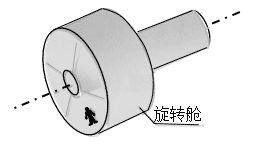
\includegraphics{figs/04.png}}

\fourchoices[answer=B]
{旋转舱的半径越大，转动的角速度就应越大}
{旋转舱的半径越大，转动的角速度就应越小}
{宇航员质量越大，旋转舱的角速度就应越大}
{宇航员质量越大，旋转舱的角速度就应越小}
%% answer: B
%% memo:
\memoanswer{
	本题原卷及材料中未提供详解，待补充。
}

\item
%% number: 5
%% paperName: 2015年天津理综第 5 题 6 分
%% typeId: 1
%% type: 单选题
%% chapter: 功和能
%% point: 整体机械能守恒
%% method: 无
%% score: 6
%% degree: 450
%% duplicateId: 0
%% body:
如图所示，固定的竖直光滑长杆上套有质量为 $m$ 的小圆环，圆环与水平状态的轻质弹簧一端连接，弹簧的另一端连接在墙上，并且处于原长状态，现让圆环由静止开始下滑，已知弹簧原长为 $L$，圆环下滑到最大距离时弹簧的长度变为 $2L$（未超过弹性限度），则在圆环下滑到最大距离的过程中\xzanswer{B}

\onepicture[h=4.2cm]{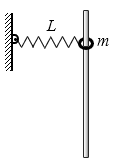
\includegraphics{figs/05.png}}

\fourchoices[answer=B]
{圆环的机械能守恒}
{弹簧弹性势能变化了 $\sqrt{3}mgL$}
{圆环下滑到最大距离时，所受合力为零}
{圆环重力势能与弹簧弹性势能之和保持不变}
%% answer: B
%% memo:
\memoanswer{
	本题原卷及材料中未提供详解，待补充。
}

\item
%% number: 6
%% paperName: 2015年天津理综第 6 题 6 分
%% typeId: 2
%% type: 多选题
%% chapter: 交流电
%% point: 变压器
%% method: 无
%% score: 6
%% degree: 450
%% duplicateId: 0
%% body:
如图所示，理想变压器的原线圈连接一只理想交流电流表，副线圈匝数可以通过滑动触头 Q 来调节，在副线圈两端连接了定值电阻 $R_{0}$ 和滑动变阻器 $R$，P 为滑动变阻器的滑动触头，在原线圈上加一电压为 $U$ 的正弦交流电，则\xzanswer{BC}

\onepicture[h=3.0cm]{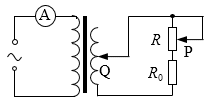
\includegraphics{figs/06.png}}

\fourchoices[answer=BC]
{保持 Q 的位置不动，将 P 向上滑动时，电流表读数变大}
{保持 Q 的位置不动，将 P 向上滑动时，电流表读数变小}
{保持 P 的位置不动，将 Q 向上滑动时，电流表读数变大}
{保持 P 的位置不动，将 Q 向上滑动时，电流表读数变小}
%% answer: BC
%% memo:
\memoanswer{
	本题原卷及材料中未提供详解，待补充。
}

\item
%% number: 7
%% paperName: 2015年天津理综第 7 题 6 分
%% typeId: 2
%% type: 多选题
%% chapter: 电场
%% point: 带电粒子的偏转
%% method: 无
%% score: 6
%% degree: 450
%% duplicateId: 0
%% body:
如图所示，氕核、氘核、氚核三种粒子从同一位置无初速地飘入电场线水平向右的加速电场 $E_{1}$，之后进入电场线竖直向下的匀强电场 $E_{2}$ 发生偏转，最后打在屏上。整个装置处于真空中，不计粒子重力及其相互作用，那么\xzanswer{AD}

\onepicture[h=3.2cm]{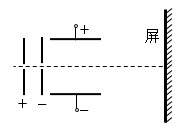
\includegraphics{figs/07.png}}

\fourchoices[answer=AD]
{偏转电场 $E_{2}$ 对三种粒子做功一样多}
{三种粒子打到屏上时速度一样大}
{三种粒子运动到屏上所用时间相同}
{三种粒子一定打到屏上的同一位置}
%% answer: AD
%% memo:
\memoanswer{
	本题原卷及材料中未提供详解，待补充。
}

\item
%% number: 8
%% paperName: 2015年天津理综第 8 题 6 分
%% typeId: 2
%% type: 多选题
%% chapter: 曲线运动
%% point: 人造地球卫星
%% method: 无
%% score: 6
%% degree: 450
%% duplicateId: 0
%% body:
$P_{1}$、$P_{2}$ 为相距遥远的两颗行星，距各自表面相同高度处各有一颗卫星 $s_{1}$、$s_{2}$ 做匀速圆周运动，图中纵坐标表示行星对周围空间各处物体的引力产生的加速度 $a$，横坐标表示物体到行星中心的距离 $r$ 的平方，两条曲线分别表示 $P_{1}$、$P_{2}$ 周围的 $a$ 与 $r^{2}$ 的反比关系，它们左端点横坐标相同。则\xzanswer{AC}

\onepicture[h=3.8cm]{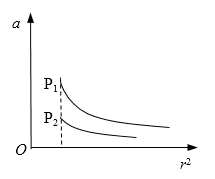
\includegraphics{figs/08.png}}

\fourchoices[answer=AC]
{$P_{1}$ 的平均密度比 $P_{2}$ 的大}
{$P_{1}$ 的“第一宇宙速度”比 $P_{2}$ 的小}
{$s_{1}$ 的向心加速度比 $s_{2}$ 的大}
{$s_{1}$ 的公转周期比 $s_{2}$ 的大}
%% answer: AC
%% memo:
\memoanswer{
	本题原卷及材料中未提供详解，待补充。
}

\item
%% number: 9
%% paperName: 2015年天津理综第 9 题 8 分
%% typeId: 4
%% type: 实验题
%% chapter: 电路
%% point: 测电动势与内阻
%% method: 无
%% score: 8
%% degree: 450
%% duplicateId: 0
%% body:
\begin{enumerate}
	\item
	如图所示，在光滑水平面的左侧固定一竖直挡板，A 球在水平面上静止放置，B 球向左运动与 A 球发生正碰，B 球碰撞前、后的速率之比为 $3:1$，A 球垂直撞向挡板，碰后原速率返回。两球刚好不发生碰撞，A、B 两球的质量之比为\tkanswer[1.5cm]{$4:1$}，A、B 碰撞前、后两球总动能之比为\tkanswer[1.5cm]{$9:5$}。

	\onepicture[h=1.6cm, align=right]{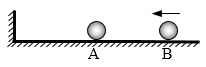
\includegraphics{figs/09a.png}}

	\item
	某同学利用单摆测量重力加速度。

	\begin{steps}
		\item
		为了使测量误差尽量小，下列说法正确的是\tkanswer[1.2cm]{BC}。

		（A）组装单摆须选用密度和直径都较小的摆球

		（B）组装单摆须选用轻且不易伸长的细线

		（C）实验时须使摆球在同一竖直面内摆动

		（D）摆长一定的情况下，摆的振幅尽量大

		\item
		如图所示，在物理支架的竖直立柱上固定有摆长约为 $1\Um$ 的单摆，实验时，由于仅有量程为 $20\Ucm$、精度为 $1\Umm$ 的钢板刻度尺，于是他先使摆球自然下垂，在竖直立柱上与摆球最下端处于同一水平面的位置做一标记点，测出单摆的周期 $T_{1}$；然后保持悬点位置不变，设法将摆长缩短一些，再次使摆球自然下垂，用同样方法在竖直立柱上做另一标记点，并测出单摆周期 $T_{2}$；最后用钢板刻度尺量出竖直立柱上两标记点之间的距离 $\Delta L$。用上述测量结果，写出重力加速度的表达式 $g=$\tkanswer[2.6cm]{$\frac{4\pi^{2}\Delta L}{T_{1}^{2}-T_{2}^{2}}$}。
	\end{steps}

	\onepicture[h=4.0cm, align=right]{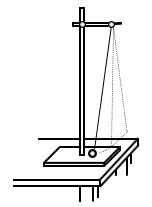
\includegraphics{figs/09b.png}}

	\item
	用电流表和电压表测定由三节干电池串联组成的电池组（电动势约为 $4.5\UV$，内电阻约为 $1\UO$）的电动势和内电阻，除了待测电池组，电键，导线外，还有下列器材供选用：

	（A）电流表：量程 $0.6\UA$，内电阻约为 $1\UO$

	（B）电流表：量程 $3\UA$，内电阻约为 $0.2\UO$

	（C）电压表：量程 $3\UV$，内电阻约为 $30\UkO$

	（D）电压表：量程 $6\UV$，内电阻约为 $60\UkO$

	（E）滑动变阻器：$0\sim1000\UO$，额定电流 $0.5\UA$

	（F）滑动变阻器：$0\sim20\UO$，额定电流 $2\UA$

	\begin{steps}
		\item
		为了使测量结果尽量准确，电流表应选用\tkanswer[0.8cm]{A}，电压表选用\tkanswer[0.8cm]{D}，滑动变阻器选用\tkanswer[0.8cm]{F}（均填仪器的字母代号）

		\item
		如图为正确选择仪器后，连好的部分电路，为了使测量误差尽量小，还需要在电路中用导线将\tkanswer[0.8cm]{a}和\tkanswer[0.8cm]{d}相连、\tkanswer[0.8cm]{c}和\tkanswer[0.8cm]{g}相连、\tkanswer[0.8cm]{f}和\tkanswer[0.8cm]{h}相连（均填仪器上接线柱的字母代号）

		\item
		实验时发现电流表坏了，于是不再使用电流表，剩余仪器中仅用电阻箱替换掉滑动变阻器，重新连接电路，仍能完成实验，实验中读出几组电阻箱的阻值 $R$ 和对应电压表的示数 $U$；用图像法处理采集到数据，为在直角坐标系中得到的函数图像是一条直线，则可以\tkanswer[1.2cm]{$\frac{1}{U}$}为纵坐标，以\tkanswer[1.2cm]{$\frac{1}{R}$}为横坐标。
	\end{steps}

	\onepicture[h=4.6cm, align=right]{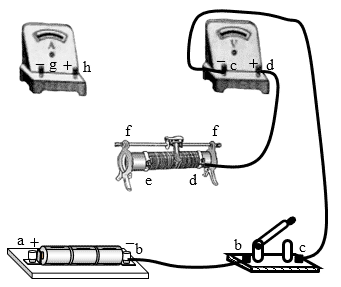
\includegraphics{figs/09c.png}}
\end{enumerate}
%% answer: 
\jdanswer{
\begin{enumerate}
	\item
	$4:1$，$9:5$

	\item
	（1）$BC$；（2）$g=\frac{4\pi^{2}\Delta L}{T_{1}^{2}-T_{2}^{2}}$

	\item
	（1）$A$，$D$，$F$；（2）$a$、$d$，$c$、$g$，$f$、$h$；（3）以 $\frac{1}{U}$ 为纵坐标、$\frac{1}{R}$ 为横坐标（或 $U$ 与 $\frac{U}{R}$、$\frac{R}{U}$ 与 $R$，横纵坐标互换亦可）
\end{enumerate}
}
%% memo:
\memoanswer{
	本题原卷及材料中未提供详解，待补充。
}

\item
%% number: 10
%% paperName: 2015年天津理综第 10 题 16 分
%% typeId: 6
%% type: 计算题
%% chapter: 运动和力
%% point: 传送带
%% method: 无
%% score: 16
%% degree: 450
%% duplicateId: 0
%% body:
某快递公司分拣邮件的水平传输装置示意图如图，皮带在电动机的带动下保持 $v=1\Ums$ 的恒定速度向右运动，现将一质量为 $m=2\Ukg$ 的邮件轻放在皮带上，邮件和皮带间的动摩擦因数 $\mu=0.5$。设皮带足够长，取 $g=10\Umsq$，在邮件与皮带发生相对滑动的过程中，求：
\begin{enumerate}
	\item
	邮件滑动的时间 $t$；

	\item
	邮件对地的位移大小 $x$；

	\item
	邮件与皮带间的摩擦力对皮带做的功 $W$。
\end{enumerate}

\onepicture[h=1.6cm, align=right]{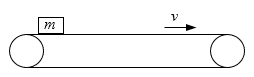
\includegraphics{figs/10.png}}

%% answer: 
\jdanswer{
\begin{enumerate}
	\item
	$t=0.2\Us$

	\item
	$x=0.1\Um$

	\item
	$W=-2\UJ$
\end{enumerate}
}
%% memo:
\memoanswer{
	（1）设邮件放到皮带上与皮带发生相对滑动过程中受到的滑动摩擦力为 $F$，则

	$F=\mu mg$\ccnum{①}

	取向右为正方向，对邮件应用动量定理，有

	$Ft=mv-0$\ccnum{②}

	由\ccnum{①}\ccnum{②}式并代入数据得

	$t=0.2\Us$\ccnum{③}

	（2）邮件与皮带发生相对滑动的过程中，对邮件应用动能定理，有

	$Fx=mv^{2}/2-0$\ccnum{④}

	由\ccnum{①}\ccnum{④}式并代入数据得

	$x=0.1\Um$\ccnum{⑤}

	（3）邮件与皮带发生相对滑动的过程中，设皮带相对地面的位移为 $s$，则

	$s=vt$\ccnum{⑥}

	摩擦力对皮带做的功

	$W=-Fs$\ccnum{⑦}

	由\ccnum{①}\ccnum{③}\ccnum{⑥}\ccnum{⑦}式并代入数据得

	$W=-2\UJ$\ccnum{⑧}
}

\item
%% number: 11
%% paperName: 2015年天津理综第 11 题 18 分
%% typeId: 6
%% type: 计算题
%% chapter: 电磁感应
%% point: 线圈过有界磁场
%% method: 无
%% score: 18
%% degree: 450
%% duplicateId: 0
%% body:
如图所示，“凸”字形硬质金属线框质量为 $m$，相邻各边互相垂直，且处于同一竖直平面内，ab 边长为 $l$，cd 边长为 $2l$，ab 与 cd 平行，间距为 $2l$。匀强磁场区域的上下边界均水平，磁场方向垂直于线框所在平面。开始时，cd 边到磁场上边界的距离为 $2l$，线框由静止释放，从 cd 边进入磁场直到 ef、pq 边进入磁场前，线框做匀速运动，在 ef、pq 边离开磁场后，ab 边离开磁场之前，线框又做匀速运动。线框完全穿过磁场过程中产生的热量为 $Q$。线框在下落过程中始终处于原竖直平面内，且 ab、cd 边保持水平，重力加速度为 $g$；求：
\begin{enumerate}
	\item
	线框 ab 边将离开磁场时做匀速运动的速度大小是 cd 边刚进入磁场时的几倍；

	\item
	磁场上下边界间的距离 $H$。
\end{enumerate}

\onepicture[h=3.8cm, align=right]{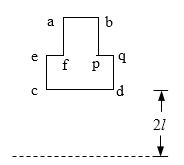
\includegraphics{figs/11.png}}

%% answer: 
\jdanswer{
\begin{enumerate}
	\item
	$4$ 倍

	\item
	$H=\frac{Q}{mg}+28l$
\end{enumerate}
}
%% memo:
\memoanswer{
	（1）设磁场的磁感应强度大小为 $B$，cd 边刚进磁场时，线框做匀速运动的速度为 $v_{1}$。

	$E_{1}=2Blv_{1}$\ccnum{①}

	设线框总电阻为 $R$，此时线框中电流为 $I_{1}$，由闭合电路欧姆定律，有

	$I_{1}=\frac{E_{1}}{R}$\ccnum{②}

	设此时线框所受安培力为 $F_{1}$，有

	$F_{1}=2I_{1}lB$\ccnum{③}

	由于线框做匀速运动，其受力平衡，有

	$mg=F_{1}$\ccnum{④}

	由\ccnum{①}\ccnum{②}\ccnum{③}\ccnum{④}式得

	$v_{1}=\frac{mgR}{4B^{2}l^{2}}$\ccnum{⑤}

	设 ab 边离开磁场之前，线框做匀速运动的速度为 $v_{2}$，同理可得

	$v_{2}=\frac{mgR}{B^{2}l^{2}}$\ccnum{⑥}

	由\ccnum{⑤}\ccnum{⑥}式得

	$v_{2}=4v_{1}$\ccnum{⑦}

	（2）线框自释放直到 cd 边进入磁场前，由机械能守恒定律，有

	$2mgl=mv_{1}^{2}/2$\ccnum{⑧}

	线框完全穿过磁场的过程中，由能量守恒定律，有

	$mg(2l+H)=\frac{1}{2}mv_{2}^{2}-\frac{1}{2}mv_{1}^{2}+Q$\ccnum{⑨}

	由\ccnum{⑦}\ccnum{⑧}\ccnum{⑨}式得

	$H=\frac{Q}{mg}+28l$\ccnum{⑩}
}

\item
%% number: 12
%% paperName: 2015年天津理综第 12 题 20 分
%% typeId: 6
%% type: 计算题
%% chapter: 磁场
%% point: 带电粒子在磁场中的运动
%% method: 无
%% score: 20
%% degree: 250
%% duplicateId: 0
%% body:
现代科学仪器常利用电场、磁场控制带电粒子的运动。在真空中存在着如图所示的多层紧密相邻的匀强电场和匀强磁场，电场和磁场的宽度均为 $d$。电场强度为 $E$，方向水平向右；磁感应强度为 $B$，方向垂直纸面向里。电场、磁场的边界互相平行且与电场方向垂直，一个质量为 $m$、电荷量为 $q$ 的带正电粒子在第 1 层电场左侧边界某处由静止释放，粒子始终在电场、磁场中运动，不计粒子重力及运动时的电磁辐射。
\begin{enumerate}
	\item
	求粒子在第 2 层磁场中运动时速度 $v_{2}$ 的大小与轨迹半径 $r_{2}$；

	\item
	粒子从第 $n$ 层磁场右侧边界穿出时，速度的方向与水平方向的夹角为 $\theta_{n}$，试求 $\sin\theta_{n}$；

	\item
	若粒子恰好不能从第 $n$ 层磁场右侧边界穿出，试问在其他条件不变的情况下，也进入第 $n$ 层磁场，但比荷较该粒子大的粒子能否穿出该层磁场右侧边界，请简要推理说明之。
\end{enumerate}

\onepicture[h=3.8cm, align=right]{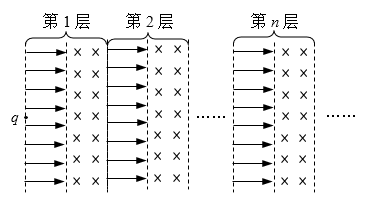
\includegraphics{figs/12.png}}

%% answer: 
\jdanswer{
\begin{enumerate}
	\item
	$v_{2}=2\sqrt{\frac{qEd}{m}}$，$r_{2}=\frac{2}{B}\sqrt{\frac{mEd}{q}}$

	\item
	$\sin\theta_{n}=B\sqrt{\frac{nqd}{2mE}}$

	\item
	若粒子恰好不能从第 $n$ 层磁场右侧边界穿出，则 $\theta_{n}=\frac{\pi}{2}$，$\sin\theta_{n}=1$，在其他条件不变的情况下，换用比荷更大的粒子，设其比荷为 $\frac{q'}{m'}$，假设能穿出第 $n$ 层磁场右侧边界，粒子穿出时速度方向与水平方向的夹角为 $\theta_{n}'$，由于 $\frac{q'}{m'}>\frac{q}{m}$，则导致 $\sin\theta_{n}'>1$，说明 $\theta_{n}'$ 不存在，即原假设不成立。所以比荷较该粒子大的粒子不能穿出该层磁场右侧边界。
\end{enumerate}
}
%% memo:
\memoanswer{
	（1）粒子在进入第 2 层磁场时，经过两次电场加速，中间穿过磁场时洛伦兹力不做功。由动能定理，有

	$2qEd=\frac{1}{2}mv_{2}^{2}$\ccnum{①}

	由式\ccnum{①}解得

	$v_{2}=2\sqrt{\frac{qEd}{m}}$\ccnum{②}

	粒子在第二层磁场中受到的洛伦兹力充当向心力，有

	$qv_{2}B=m\frac{v_{2}^{2}}{r_{2}}$\ccnum{③}

	由\ccnum{②}\ccnum{③}式解得

	$r_{2}=\frac{2}{B}\sqrt{\frac{mEd}{q}}$\ccnum{④}

	（2）设粒子在第 $n$ 层磁场中运动的速度为 $v_{n}$，轨迹半径为 $r_{n}$（各量的下标均代表粒子所在层数，下同）。

	$nqEd=\frac{1}{2}mv_{n}^{2}$\ccnum{⑤}

	$qv_{n}B=m\frac{v_{n}^{2}}{r_{n}}$\ccnum{⑥}

	粒子进入第 $n$ 层磁场时，速度的方向与水平方向的夹角为 $\alpha_{n}$，从第 $n$ 层磁场右侧边界穿出时速度方向与水平方向的夹角为 $\theta_{n}$，粒子在电场中运动时，垂直于电场线方向的速度分量不变，有

	$v_{n-1}\sin\theta_{n-1}=v_{n}\sin\alpha_{n}$\ccnum{⑦}

	由图 1 可得

	$r_{n}\sin\theta_{n}-r_{n}\sin\alpha_{n}=d$\ccnum{⑧}

	\onepicture[showlabel=false, align=right, h=4.2cm]{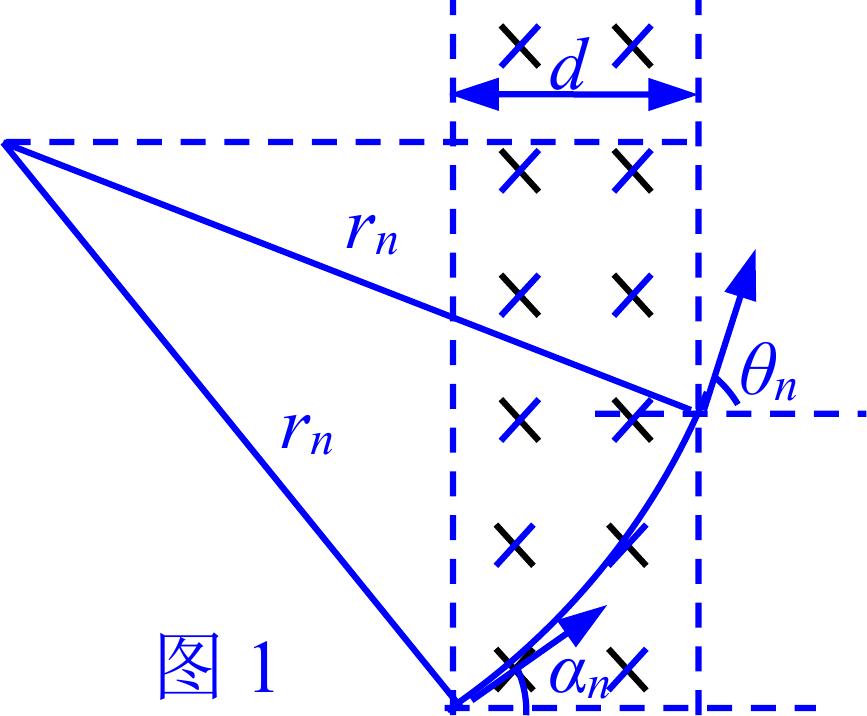
\includegraphics{figs/12b.png}}

	由\ccnum{⑥}\ccnum{⑦}\ccnum{⑧}式得

	$r_{n}\sin\theta_{n}-r_{n-1}\sin\theta_{n-1}=d$\ccnum{⑨}

	由\ccnum{⑨}式看出 $r_{1}\sin\theta_{1}$，$r_{2}\sin\theta_{2}$，$\cdots$，$r_{n}\sin\theta_{n}$ 为一等差数列，公差为 $d$，可得

	$r_{n}\sin\theta_{n}=r_{1}\sin\theta_{1}+(n-1)d$\ccnum{⑩}

	当 $n=1$ 时，由图 2 可得

	$r_{1}\sin\theta_{1}=d$\ccnum{⑪}

	\onepicture[showlabel=false, align=right, h=4.2cm]{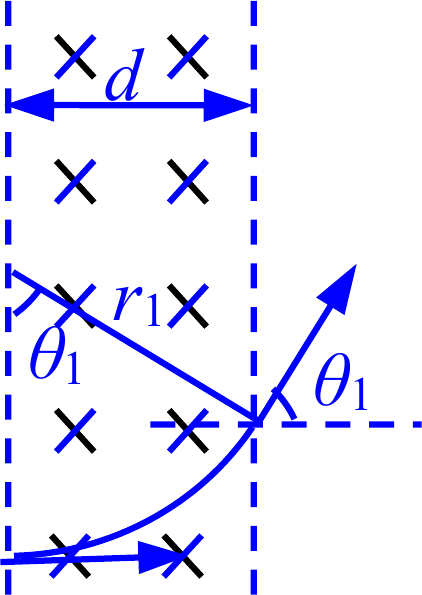
\includegraphics{figs/12c.png}}

	由\ccnum{⑤}\ccnum{⑥}\ccnum{⑩}\ccnum{⑪}式得

	$\sin\theta_{n}=B\sqrt{\frac{nqd}{2mE}}$\ccnum{⑫}

	（3）若粒子恰好不能从第 $n$ 层磁场右侧边界穿出，则 $\theta_{n}=\frac{\pi}{2}$，$\sin\theta_{n}=1$，在其他条件不变的情况下，换用比荷更大的粒子，设其比荷为 $\frac{q'}{m'}$，假设能穿出第 $n$ 层磁场右侧边界，粒子穿出时速度方向与水平方向的夹角为 $\theta_{n}'$，由于 $\frac{q'}{m'}>\frac{q}{m}$，则导致 $\sin\theta_{n}'>1$，说明 $\theta_{n}'$ 不存在，即原假设不成立。所以比荷较该粒子大的粒子不能穿出该层磁场右侧边界。
}

\end{enumerate}

\end{document}
